\chapter{Discussion and Conclusions}\label{ch:conclusion} % Main chapter title

\section{Summary of the application of our results to \GW{}}

In this chapter we summarize how the results discussed in this thesis 
provide additional information on the \GW{}, the only \ac{BNS} merger 
observed so far in \ac{GW} and \ac{EM} spectra.


\begin{figure*}[t]
    \centering 
    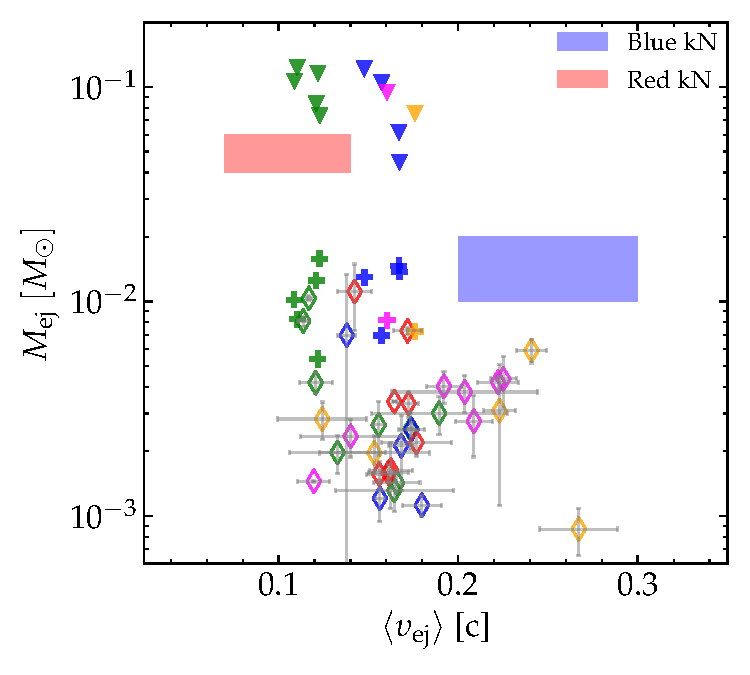
\includegraphics[width=0.48\textwidth]{ejecta_dyn/summary/ej_mej_vej_our2.pdf}
    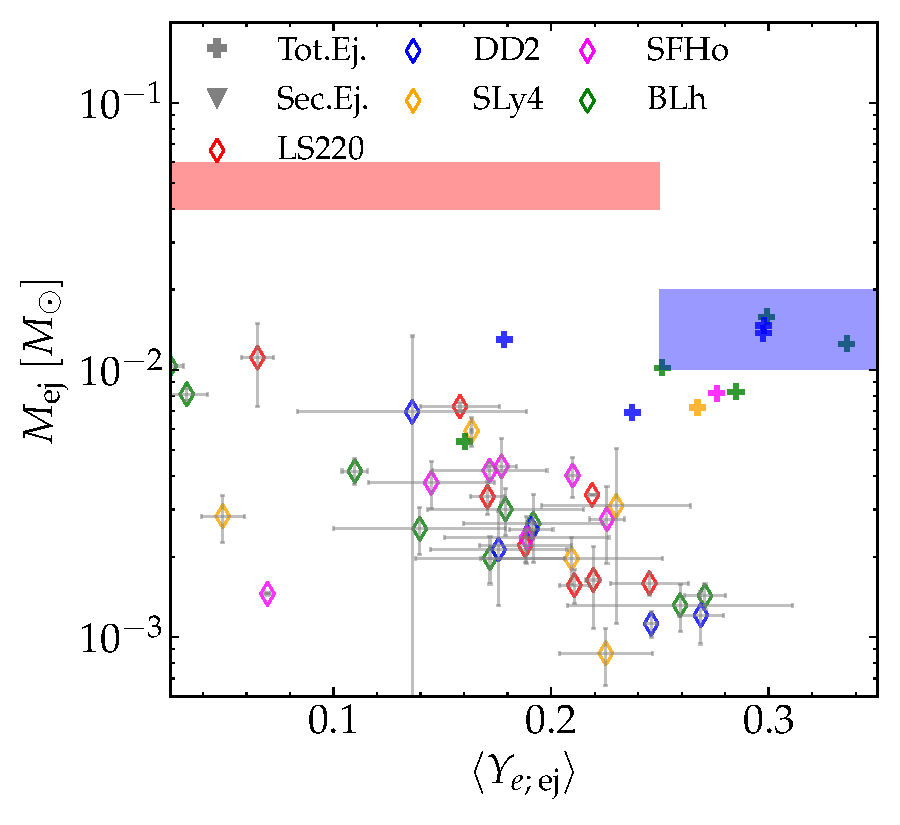
\includegraphics[width=0.48\textwidth]{ejecta_dyn/summary/ej_mej_yeej_our2.pdf}
    \caption{
        Summary of the ejecta properties of our models.
        %
        Diamonds mark the dynamical ejecta, crosses include the
        contribution of the \swind{} for the long-lived models, 
        triangles are an estimate of the total ejecta mass on a secular
        timescale, assuming $40\%$ of the disk mass is unbounded on
        secular timescales.         
        The ejecta mass is shown is terms of the mass-averaged velocity
        (left) and of the averaged electron fraction (right).
        %
        The filled blue and red patches are the expected values of
        ejecta mass and velocity for blue and red components of
        AT2017gfo compiled by \cite{Siegel:2019mlp}, based on
        \cite{Villar:2017wcc}. 
        Adopted from \citet{Nedora:2020pak}.
    }
    %
    \label{fig:ejecta:dyn:ds_sww}
\end{figure*}


%% from main paper, referencing the fitpaper Poly22 fits and SWW + DE
%\red{THis can be augmented with Radio afterglow}

%% === FROM DYNAMICAL EJECTA SECTION of MAIN PAPER
%Here we discuss the application of our results to \GW{}.


\subsection{Dynamical Ejecta}

%In Chapter~\ref{ch:bns_sims}, Sec~\ref{}

The properties of the dynamical ejecta from the \ac{BNS} mergers are of key 
importance to determine the properties of the \ac{EM} counterpart. 
%
In Chapter~\ref{ch:bns_sims}, Sec~\ref{sec:bns_sims:dyn}, we examined the mass, 
velocity and electron fraction of the \ac{DE} from our simulations and showed 
that they can be mapped back onto the inital properties of the binary, \ie, 
\mr{} and $\tilde{\Lambda}$, via a simple two parameter polynomial, \polql{}. 
%
We further explore this and other fitting formulae and assess their effectiveness 
when \ac{NR} simulations from different groups with different physics input are 
considered in Appendix~\ref{ch:stat}.
%


%The \GW{} is the only \ac{BNS} merger observed as a \mm{} event, observed so far.
%
%
%%% ---
%First, we asses the ejecta parameters that our fitting models, 
%obtained in section \ref{sec:ejecta_disk_statisitcs} would provide for the \GW{}.
%% --- 
The properties of \GW{} system, from LIGO-Virgo \ac{GW} analysis, 
\citep{TheLIGOScientific:2017qsa,Abbott:2018wiz,De:2018uhw,Abbott:2018exr} \ie, 
$90\%$ credible intervals estimated for $q$ and $\tilde{\Lambda}$ 
are
$\tilde{\Lambda}=300_{-190}^{+500}$ and $q\in[1., 1.37]$. 
%and using the errorbars formulas developed in \cite{Radice:2018pdn}, we find that
Applying the \polql{} fitting formula %, calibrated with the \DSrefset{} 
to the \GW{} parameters we obtain:
%
$\amd \in [0.72, 7.52] \times 10^{-3}\, M_{\odot}$
and
$\avd \in [0.16, 0.39]\,$c 
and 
$\ayd \in [0.11, 0.23]$.
%
Notably, these values do not agree with those inferred for \AT{} by the spherical, 
two-component \ac{kN}. models \citep{Villar:2017wcc} and further underlines the 
importance of the geometry in modeling \ac{kN}, as we discussed in Ch.~\ref{ch:kilonova}.


Analysis of a set of \ac{kN} fitting models provides a broad range of ejecta 
parameters \citep{Siegel:2019mlp}:
%
$M_{\text{ej}}^{\text{red}}\in(4, 6)\times10^{-2}\,M_{\odot}$ and
$\upsilon_{\text{ej}}^{\text{red}}\in(0.07, 0.14)\,c$ for the red component, while
$M_{\text{ej}}^{\text{blue}}\in[1, 2]\times10^{-2}\,M_{\odot}$ and 
$\upsilon_{\text{ej}}^{\text{blue}}\in[0.2, 0.3]\,c$ for the blue component.
%
With respect to our results for \ac{DE}, however, 
none of the \ac{kN} components can be well explained.

In Fig.~\ref{fig:ejecta:dyn:ds_sww} we show the ejecta properties from our 
models and the parameters inferred from the
observations as red and blue boxes. 
%
With respect to the red component, we observe that \ac{DE} from our models 
have too high average velocities and not nearly enough mass.
This result suggests that an additional, low $Y_e$ ejecta component is required
in order to explain the \AT{} red component 
\citep{Perego:2017wtu,Kawaguchi:2018ptg,Nedora:2019jhl}.
%
A more thorough analysis of the \AT{} with better ejecta models and advanced
radiation transport kilonova simulations are not part of the present work 
and will be addressed in the future.

The analysis of the \ac{kN} non-thermal afterglow, Ch.~\ref{ch:afterglow}, 
cannot provide conclusive constraints on the properties of \ac{DE} yet. 
We can only note, that as the mild ejecta velocities seems to be preferred by the 
emerging new \GRB{} afterglow component, the emitting material had contributed 
to the red component of the \ac{kN} primarily.
%
Significantly more observational data is required for linking the \ac{kN} and 
its afterglow to ejecta properties and ultimately to the properties of the 
binary are required.



\subsection{Spiral-wave wind}

Discussing the \ac{BNS} models' merger dynamics and mass ejection we identified 
a new ejecta component, driven by the interaction between the \ac{NS} merger 
remnant and the disk, the \ac{SWW} (Ch.~\ref{ch:bns_sims}, Sec.~\ref{sec:bns_sims:dyn}).
We showed that this ejecta is more massive than \ac{DE}, if the \ac{NS} remnant 
is long-lived, and has high electron fraction (Sec.~\ref{sec:bns_sims:sww}).
%
The \ac{SWW} could be a significant contributor to the \AT{}, assuming the remnant 
of \GW{} \ac{MNS} merger survived for $\mathcal{O}(100)$~ms, as we showed 
in Ch.~\ref{ch:kilonova}, Sec.~\ref{sec:kilonova:result}.


In Fig.~\ref{fig:ejecta:dyn:ds_sww} we report the total (dynamical+\swind{}) ejecta 
mass and mass-averaged velocity for the simulated long-lived \ac{BNS} (crosses).
%
Notably, the total ejecta mass of three of our models, 
BLh $q=1.18$, BLh $q=1.42$ and DD2 is $q=1.00$ are in agreement with the expected 
values for the blue component of \AT{}.
%(obtained using the two-component fit \citep{Villar:2017wcc})

The high electron fraction of the \ac{SWW} %(see Sec.~\ref{sec:bns_sims:sww}) 
however would result in a lanthanides-poor composition of the outflow 
(Sec.~\ref{sec:nucleo:results}). Thus, the \ac{SWW} cannot explain the 
observed emission for the high opacity, lanthanides-rich material.
%
Simulations with advanced physics of a \ac{MNS} mergers on a timescales 
${>}100\,$ms are required to asses the contribution from other outflow mechanisms, 
\citep{Lee:2009uc,Fernandez:2015use,Siegel:2017nub,Fujibayashi:2017puw,Fernandez:2018kax,Radice:2018xqa}.



\subsection{Secular Ejecta}

On the timescale of seconds, much longer than the evolution of our simulations 
the nuclear recombination can unbind a fraction of the disk mass 
(See Sec.~\ref{sec:bns_sims:mj_loss} for more details). % See Mb-J plot for example
%
Analytical estimates and simulations with various approximations show that up tp ${\sim}40\%$ 
of the disk can be ejected via viscous processes with an typical velocity ${\lesssim}0.1\,$c
\citep{Lee:2009uc,Fernandez:2015use,Wu:2016pnw,Siegel:2017nub,Fujibayashi:2017puw,Fernandez:2018kax,Radice:2018xqa,Fujibayashi:2020dvr}.
%
Adapting the constant fraction of the $40\%$ of the $M_{\rm disk}$, we estimate 
that about ${\sim}0.05\, M_{\odot}$ would be ejected in a form of 
secular winds. We adopt this evaluation for every simulation with the long-lived 
\ac{MNS} remnant in Fig.~\ref{fig:ejecta:dyn:ds_sww} (lower triangles).
%
We observe that the estimated mass is sufficient to explain the red component of 
\AT{}, as inferred from the two-components \ac{kN} models of \citep{Villar:2017wcc}. 








%% ---------------------
%Sources with time delay are preferred by studies of very metal poor stars that indluded the time delay for r-process elements
%to diffuse through ISM, \citep{Tarumi:2021xvw}. 
%A winds from proto-nuetron are also contributors to the $r$-process budget \cite{Vincenzo:2021rvw}
%
%\red{The remnant is losing anular momentum while disk gains on shortly after merger is due to gravitational torque \cite{Shibata:2019wef}}
%








\section{Conclusion}

%% =======================================================
%%
%%                   Conclusion
%%
%% =======================================================


The scope of this thesis was to advance our understanding of the \ac{BNS} mergers,
and fundamental physics, by using the state-of-the-art \ac{NR} simulations with
advanced physics and \ac{EM} models in tandem with \mm{} observations of the 
\GW{}. 



%% \section{Conclusion}

%In this part we discussed the long-term dynamics of the $37$ \ac{BNS} merger simulations
%focusing on the long-term evolution and hydrodynamics. 
%The binaries span the range total mass $M\in[2.73, 2.88]\,\Msun$, 
%mass ratio $q\in[1,1.8]$, and had fixed chirp mass $\mathcal{M}_c=1.188\,\Msun$.
%We considered five microphysical \ac{EOS} compatible with the current nuclear and
%astrophysical constraints. 
%%% ---
%Each \ac{BNS} model was computed at several resolutions. 
%In total $76$ simulations were considered, some of which were ${\sim}100$~ms 
%long. Together with our previous data
%\citep{Bernuzzi:2015opx,Radice:2016dwd,Radice:2016rys,Radice:2017lry,Radice:2018xqa,Radice:2018pdn,Perego:2019adq,Endrizzi:2019trv,Bernuzzi:2020txg}
%these simulations form the largest sample of merger simulations with microphysics
%available to date. 
%\red{Our ejecta data are publicly available \citep{vsevolod_nedora_2020_4159619}.
%}

%\subsection{Disk \& Remnant}

Considering the \pmerg{} evolution of \ac{BNS} merger remnant, we find an
overall strong dependency on the system \mr{} and \ac{EOS}, and on the 
finite temperature effects in the latter. One of the key affected 
parameters is the remnant lifetime. We find that models with 
soft \acp{EOS} or/and large \mr{}s produce short-lived \ac{NS} remnants that 
collapse within few ${\sim}10\,$ms after merger. 
%
More symmetric models with stiffer \acp{EOS} produce long-lived, possibly 
stable remnants. The lifetime of the \ac{NS} remnant appears to be correlated with the 
disk mass for the $q\sim 1$ models, in agreement with previous findings 
\citep{Radice:2017lry,Radice:2018pdn}.
Binaries with larger \mr{}s tend to have more massive disks and more massive tidal 
compoents of the \ac{DE}.
%
%The disk temperature and composition show dependency on the \mr{}. For instance, 
%models with $q{\sim}1$ form a disk primarily from the material squeezed out at the 
%\acp{NS} collisional interface. Such disk is characterized by relatively high 
%temperatures $O(10\, {\rm MeV})$. Its composition evolves from being 
%relatively proton reach, with electron fraction set by the 
%neutrino irradiation and shocks to $Y_e \simeq 0.25$, to being neutron rich with 
%$Y_e\simeq0.1$ as disks settles on a quasi-steady state. 
%This is in agreement with the theory of neutrino dominated accretion 
%flows \citep{Beloborodov:2008nx,Siegel:2017jug}. 
%
The long-term evolution of the \ac{NS} remnants is governed by both accretion, 
induced by the neutrino cooling and viscous stresses, and mass shedding that originates 
in gravitational and hydrodynamical torques and neutrino reabsorption (heating).
%\citep[spiral waves][]{Radice:2018xqa}
Our simulations show that the newly formed \ac{NS} remnant with mass exceeding the 
maximum of the uniformly rotating configuration (so-called \ac{HMNS}) does 
not necessarily collapse to a \ac{BH}. Instead, massive winds, such as \ac{SWW}
found in our simulations, can 
efficiently remove the excess in mass (alongside the angular momentum), bringing 
the \ac{NS} remnant to a rigidly rotating configuration.
%
%In order to asses the ultimate fate of the \ac{BNS} mergers with masses that fall 
%in-between the maximum for a nonrotating \ac{NS} and those leading to a prompt collapse,
%the long-term $3$D neutrino-radiation \ac{GRMHD} simulations are required.

Considering the matter ejected during and after mergers, we find 
two distinct types. The \ac{DE} and the \pmerg{} \ac{SWW}. 
%% --- dynamical
With respect to the former, we extend the previous analysis done by \citet{Radice:2018pdn} 
with 
more advanced physics input and larger parameter space of our models.
We further extend our analysis by considering the ejecta properties 
statistics across different \ac{NR} simulations with various physics inputs 
and identify simple mapping from ejecta properties to the 
binary properties.
%
%(i) consistent inclusion of neutrino reabsorption via the M0 scheme,
%(ii) addition of the effects of the \ac{MHD} turbulence in most simulations 
%via the \ac{GRLES} subgrid model, 
%(iii) direct focus on the \GW{} with all models having corresponding chirp mass,
%whilst still considering models with larger \mr{} than in the aforementioned study.
%We also augment the analysis of our own simulaltions with the largest-to-date compiled
%set of \ac{BNS} merger simulations in the literature. 
%
We find that the neutrino reabsorption has a systematic effect on the \ac{DE} properties.
Its inclusion raises the ejecta mass and velocity.
%This result is in agreement with previous studies \citep{Sekiguchi:2015dma,Radice:2018pdn}.
The ejecta electron fraction, elevated by the neutrino reabsorption, is similar to that 
found in simulations with different approximation schemes for neutrinos
\citep{Sekiguchi:2016bjd,Vincent:2019kor}. 
This suggests that the current neutrino schemes in \ac{NR} simulations are able to 
reproduce the main neutrino effects consistently.
%Our set of simulations shows that the properties of the \ac{DE} depend on the \mr{}.
We also find that the ejecta velocity and electron fraction decrease with \mr{}, while 
the total mass increases. However the statistical significance of the latter is weak.

%% --- SWW
In cases where \ac{NS} merger remnant is long-lived, we identify a new ejecta component, 
the \ac{SWW}. This wind is driven by the energy and angular momentum injected into the 
disk by the remnant, subjected to the bar-mode and one-armed dynamical instabilities.
%that are present in \ac{MNS} remnants formed in mergers
%\citep{Shibata:1999wm,Paschalidis:2015mla,Radice:2016gym}
We find that within the simulation time, (up to ${\sim}100$~ms) the \ac{SWW} does not 
saturate, unless the \ac{NS} remnant collapses to a \ac{BH}.
%The mass-loss rate via the \ac{SWW} is ${\sim}0.1{-}0.5\, \Msun\, {\text{s}}^{-1}$.
The \ac{SWW} have a broad distribution in electron fraction, being on average higher,
then that of the \ac{DE}, and narrow distribution in velocity, and can unbind
${\sim}0.1{-}0.5\, \Msun$ within a second.
%% --- Nu-Wind
A part of the \ac{SWW}, channeled along the polar axis and exhibiting the highest
electron fraction we identify as \nwind{}. Contrary to other studies of the 
neutrino-driven outflows, \citep[\eg][]{Dessart:2008zd,Perego:2014fma,Fujibayashi:2020dvr}
the \nwind{} in our simulations saturates shortly after merger.
%
%However, while in the early \pmerg{} 
%tje properties of the \nwind{} in our simulations are similar to that found in the 
%\citet{Dessart:2008zd,Perego:2014fma,Fujibayashi:2020dvr}, within few tens 
%of milliseconds after merger as polar region above \ac{MNS} remnant 
%becomes polluted by the material lifted from the disk by thermal pressure. 
Notably, the steady state $\nu$-wind is generally referred to the outflow 
that emerges on a timescale of hundreds of milliseconds, longer than ours. Additionally, it is 
plausible, that the approximated neutrino reabsorption scheme used in our 
simulations is insufficient in this case. 
Long-term simulations employing more advanced 
neutrino transport schemens are requred to asses the properties of the \nwind.
%In the early \pmerg{}, the properties 
%of the wind are similar to $\nu$-wind found in 
%\eg~\citet{Dessart:2008zd,Perego:2014fma,Fujibayashi:2020dvr}.
%However, in our simulations the \nwind{} mass flux saturates within few tens 
%of milliseconds after merger, as polar region above \ac{MNS} remnant 
%becomes polluted by the material lifted from the disk by thermal pressure. 
%Notably, the emergence of the steady state $\nu$-wind is generally associated 
%with longer timescales that those, simulated here. It is thus possible, that the 
%conditions for the onset of \nwind{} have not been achieved in our simulations.
%Additionally, it is possible that the approximate neutrino treatment 
%employed in our simulations is not sufficient. 
%The emergence of the \nwind{} should be further investigated with long-term 
%simulations employing more advanced neutrino transport schemens.
%
Additionally, the effects of magnetization are important for the polar outflow 
\citep{Siegel:2017nub,Metzger:2018uni,Fernandez:2018kax,Miller:2019dpt,Mosta:2020hlh}.
Our simulations do not include magnetic fields and thus we cannot asses their 
effect on the outflow. However, the simulations include turbulent viscosity 
that have been show to produce a similar effect on the bulk of the secular 
outflow to the full-\ac{MHD} \citep{Fernandez:2018kax}.

%% --- Nucleo
We asses the outcome of \rproc{} \nuc{} in the ejected matter via the precomputed 
parameterized model, based on the \ac{NRN} \texttt{SkyNet} \citep{Lippuner:2015gwa}.
%
The \rproc{} in \ac{DE} depends strongly on \mr{}, following the electron fraction,
with large amount of lanthanides and actinides produced in high-$q$ cases.
%We find that as the \ac{DE} electron fraction depends on the binary \mr{}, so do the 
%\rproc{} yields. For instance, the ejecta from binaries with large $q$ is very neutron-rich 
%and the nucleosynthesis in it produces large amount of lanthanides and actinides.
Binaries with the highest \mr{} considered, that undergo prompt collapse, show the 
actinides abundances similar to solar.
Binaries with $q \sim 1$ produce less neutron-rich \ac{DE} and the 
final abundances show significant production of lighter elements,
%Ejecta from binaries with small $q{\sim}1$, on the other hand, is less neutron-rich 
%and the final abundances show significant production of lighter elements.
If the merger remnant is a \ac{NS}, the final \rproc{} abundances in the ejecta 
(that include \ac{DE} and \ac{SWW}) show large amount 
of both heavy and light elements produced. 
We observe that the abundance pattern in the total ejecta 
is similar to solar down to the $A\simeq 100$.
This result further implies the importance of \ac{BNS} mergers in cosmic 
chemical evolution.

%% Kilonova
%We compute the \ac{kN} emission from the decay of \rproc{} elements in ejecta using 
%the semi-analytic, anisotropic, multi-component model with nuclear heating rates 
%and opacities inferred from dedicated studies.
Considering the thermal emission from the decay of \rproc{} elements in ejecta, \ac{kN}, 
from our models with find that, when spherically symmetric \ac{kN} models are 
considered \citep{Villar:2017wcc}, none of our models can explain 
the \AT{} bolometric light curves.
However, when an anisotranisotropic multi-components \ac{kN} models are considered, 
that take into account properties and geometry of ejecta, 
certain key features of \AT{} are recovered.
Specifically, we find that the early blue emission can be explained 
when both \ac{DE} and \ac{SWW} are considered for a binary with long-lived \ac{MNS} remnant.
However, high electron fraction material was also shown to be present in the outflows 
from \ac{BH}-torus systems and thus does not necessarily require a long-lived \ac{NS} 
\citep{Fujibayashi:2020qda}.
The late time red kilonova component requires massive, ${\sim}20\%$ of the disk mass, 
low-$Y_e$ outflows. Such outflows can be driven by viscous processes and nuclear recombination 
on a timescale of seconds \citep[\eg][]{Metzger:2008av}.
%The presence of the high electron fraction, low opacity massive outflow, \ac{SWW} 
%eases the tension found between the \ac{kN} models applied to \AT{} and \ac{NR} 
%simulations, especially with respect to the early blue emission. And while other 
%interpretation exists they are not free from internal inconsistencies. 
%Standard kN models applied to the early AT2017gfo light curve are in
%tension with ab-initio simulations conducted so far.
%While alternative interpretations have been proposed, they are either
%disfavored by current simulations and observations (e.g. jets) \citep{Bromberg:2017crh,Duffell:2018iig},
%or require the presence of large-scale strong magnetic 
%fields which might not be formed in the postmerger
%\citep{Metzger:2018uni,Fernandez:2018kax,Radice:2018ghv,Ciolfi:2019fie}. 
%We identified a robust dynamical mechanism for mass ejection that
%explains early-time observations without requiring any fine-tuning.
%The resulting nucleosynthesis is complete and produces all
%$r$-process elements in proportions similar to solar system abundances.
%Methodologically, our work underlines the importance of employing
%NR-informed ejecta for the fitting of light-curves.
%Meanwhile, the \ac{SWW} of robust dynamical origin provides a natural explanation
%without requiring model fine-tuning and underlines the \ac{NR}-informed ejecta for 
%the fitting of light-curves.
%
%Further work in this direction should 
%include better neutrino-radiation transport and magnetohydrodynamic effects
%\citep{Siegel:2017nub,Fujibayashi:2017puw,Radice:2018xqa,Radice:2018pdn,Miller:2019dpt}. 
%\red{The dependency of the ejecta properties on the binary parameters can be used 
%    in the \ac{kN} parameter estimation. We asses this possibility and provide the 
%    updated statistical investigations of the ejecta properties in the section \ref{sec:ejecta:statistics}}.

% Kilonova Afterglow
Considering the synchrotron afterglow from the interaction between the cold  ejecta and 
\ac{ISM}, we find that the recently observed change in the the afterglow of \GRB{} behaviour 
at $10^3$~days can be explained by the \ac{kN} afterglow produced by ejecta in 
ab-initio \ac{NR} \ac{BNS} simulations targeted to \GW{}. 
%
Specifically, models with moderately stiff \acp{EOS} and moderately large \mr{}, 
that produce a mild amount of fast ejecta, are favored.
%
Our results are subjected to uncertainties, the dominant among which are introduced 
by ill-constrained microphysical parameters. 
Additionally, the systematic effects due to the finite resolution, neutrino treatment 
and \acp{EOS} might be important. 
%%
%A larger set of observations, that allows for a better assessment of shock microphysics, 
%and a larger sample of high resolution \ac{NR} simulations are required to investigate 
%these uncertainties further. We leave this to future works.

%% --- Targeted to GW 170817
%Comparing the ejecta properties from our simulations to those, iferred from the 
%fitting of \AT{} bolometric light curves \citep{Villar:2017wcc}, 
%we observe that none of our models is sufficient. 
%However, when an anisotranisotropic multi-components kilonova models, iformed by the 
%ejecta properties and geometry are employed, certain key features of \AT{} are recovered.
%Specifically, we find that the early blue emission can be explained 
%when both \ac{DE} and \ac{SWW} are considered for a binary with long-lived \ac{MNS} remnant.
%However, high electron fraction material was also shown to be present in the outflows 
%fron \ac{BH}-torus systems and thus does not requires a long-lived \ac{MNS} 
%\citep{Fujibayashi:2020qda}.
%The late time red kilonova component requires massive, ${\sim}20\%$ of the disk mas, 
%low-$Y_e$ outflows. Such outflows can be driven by viscous processes and nuclear recombination 
%on a timescale of seconds \citep[\eg][]{Metzger:2008av}.

%% --- overall conclusion :: loocing forward
\paragraph{Future work}

In order to investigate the \pmerg{} dynamics in more detail: 
(i) asses the remnant lifetime and the ultimate fate, 
(ii) verify the presence of the \ac{SWW} and \nwind{} and their properties,
more simulations are required. 
%
Specifically, 
high resolution long-term (several seconds) $3$D neutrino-radiation \ac{GRMHD} 
simulations, computed with advanced microphysical \acp{EOS} with finite temperature effects.
This might become possible as new, more advanced \ac{NR} codes become available 
\citep[\eg][]{Daszuta:2021ecf}.
Special attention should be given to the neutrino treatment methods as they affect strongly the 
properties and composition of ejecta.
Several methods that are now in development, such as gray or spectral M1 \citep{Foucart:2016rxm,Roberts:2016lzn},
or Monte-Carlo methods, are steps in the right direction. Current leakage-based schemes, such as 
the M0 scheme used in this thesis and M1-leakages scheme of \citet{Sekiguchi:2015dma,Fujibayashi:2017puw}
cannot adequately treat the diffusion of neutrinos from the interior of the
\pmerg{} \ac{NS} remnant.
Additionally, the \ac{MHD} effects need to be re-examined. While it is 
apparent that \ac{MHD} is crucial for launching the relativistic jet, its effects on the 
ejecta and nucleosynthesis is not yet clear \citep{Siegel:2017jug, Fernandez:2018kax}.

On the other front, the growing number of observational facilities and their increasing 
sensitivity requires continuous advancement in models of \ac{EM} counterparts to mergers.
%
For instance, while \ac{EM} follow-up of \GW{} started ${\sim}11\,$hours after the \ac{GW} 
trigger and very early emission was not observed, if observed in future events, 
it can provide very important information on the event. 
Specifically, the prompt $\gamma$-ray emission from \ac{SGRB} allows to 
gauge the energetics of the event and geometry of the system.
Additionally, the UV-precursor emission, can hint the presence of the very 
fast ejecta component. 
%
With respect to the \ac{kN} models the attention needs to be given to the (i) geometry 
of the ejecta (ii) dynamical evolution of the ejecta (iii) non-\ac{LTE} effects.
The latter are epsecially important as with the launch of \ac{JWST}, the late \ac{kN} 
emission in \ac{IR} band would become observable for an event in the 
relative vicinity.
% 
Considering the \ac{GRB} afterglow modeling, the link between the \ac{BNS} system 
and the properties of the collimated ejecta (and ultimatelly to the afterglow) is 
required. Similar situation is with the \ac{kN} afterglow modeling.
%
Next, several processes in the pre-merger and post-merger stages of the 
\ac{BNS} system can produce \ac{EM} signals that could be their 
respective 'smoking guns'. 
For instance, the \ac{EM} emissions from inspiraling strongly magnetized \acp{NS} 
\citep[\eg][]{Beloborodov:2020ylo}, fall-back accretion onto a \ac{BH} \citep[\eg][]{Desai:2018rbc}
and \ac{NS} \citep[\eg][]{Gibson:2017dep}.
%

Finally, 
combining all the aforementioned methods and models would result in a 
surrogate \ac{EM} model of \ac{BNS} mergers that in tandem with 
already actively developing surrogate \ac{GW} models would allow for 
fast and accurate inference of binary properties.
%
An example of such model is the \texttt{NMMA} pipeline \citep{Dietrich:2020efo} that 
was recently used to provide the constant on the $R_{1.4}$, incorporating data from 
nuclear physics, pulsar observations and \GW{}.

Rapidly growing sample of observed \ac{BNS} mergers in \acp{GW} and \ac{EM} in the next few 
years with provide an unprecedented amount of information that would requrie constant 
re-analysis with advancing models, techniques and our understanding of the merger process.
It is a formidable challenge, that would benefit from state-of-the-art tools and methods, 
such as machine learning. 
%


%Finally, to infer the binary parameters and \ac{NS} \ac{EOS}, the \mm{} studies, that 
%bring together the state-of-the-art \ac{NR} simulations and \ac{EM} counterpart models are
%required. Such are the \texttt{NMMA} pipeline \citep{Dietrich:2020efo} that was recently
%used to provide the constant on the $R_{1.4}$, incorporating data from nuclear physics, 
%pulsar observations and \GW{}.
%
%
%Further work is required to overcome the limitations of this study.
%In order to asses weather the \AT{} \red{and its afterglow} can be explained from the 
%first principles, the long-term (several seconds), \ac{NR} \ac{BNS} merger simulations
%are required. Special attention should be given to the neutrino treatment, and more 
%accurate transport schemes, such as gray or spectral M1 \citep{Foucart:2016rxm,Roberts:2016lzn},
%or Monte-Carlo methods are required. Current methods leakage-based schemes, such as 
%the M0 scheme used in this work and M1-leakages scheme of \citet{Sekiguchi:2015dma,Fujibayashi:2017puw}
%cannot adequately treat the diffusion of neutrinos from the interior of the \ac{MNS} remnant.
%Additionally, the \ac{MHD} effects needs to be re-examined. While it is 
%apparent that \ac{MHD} is crucial for launching the relativistic jet, its effects on the 
%ejecta and nucleosynthesis is not yet clear \citep{Siegel:2017jug, Fernandez:2018kax}.
%
%
%Future work \& other counterparts \& MM pipeline \& PI and inference
%
%%
%In a high velocity tale of the \ac{DE}, the neutrons might avoid being captuired on a seed nuclide and freely 
%decay, producing a short, a few hours, and bright \ac{UV} precursor \citep{Metzger:2014yda}. 
%Unfortunately, in case of \AT{}, the \ac{EM} followup started \red{11} hours after the \ac{GW} detection.
%%
%See Figure 6 from \cite{Metzger:2016pju} for an examples of lightcurves of Kilonova and precursor.